\chapter{连续型机械臂的研究现状}
	\section{连续型机械臂的发展历程}
%	介绍,应用场景、历史发展、连续型机器人的概念。

受自然界象鼻、章鱼腕足、藤蔓等柔性组织或结构的启发,很多研究团队针对连续型机器人展开了深入广泛的研究。与传统的由刚性臂杆及刚性关节构成的机器人相比, 连续型机器人具有很强的灵活性和内在的柔顺性,因此在航空航天\cite{walker_robot_2013}、微创手术(MIS) \cite{conrad_interleaved_2017,gilbert_elastic_2016} 等领域获得了越来越多研究者的关注。
 
连续型机器人的概念首先由Robinson等人提出\cite{robinson_continuum_1999},他们认为连续型机器人是能够通过弹性变形沿长度方向连续弯曲,产生光滑的曲线来实现运动的一类新型机器人。宽泛的讲,连续型机器人的决定性特征是具有能够连续变化的支撑结构,并且这种结构富有柔顺性。因此,由小段刚性模块和整体弹性支撑构成的超冗余机器人,其在一定程度上具有连续型柔性臂的特征。但从严格意义上讲,这类超冗余串联机器人并不属于连续型机器人,因为它们只能产生近似连续曲率的空间曲线。一些学者为了严格划分,将这类模块化结构组成的超冗余机器人称为“连续风格(continuum-style)”机器人\cite{walker_continuous_2013}和“类连续型(pseudocontinuum robot)机器人”\cite{burgner-kahrs_continuum_2015}等。
%	实际上,连续型机器人具有无限多自由度,而上述类连续型机器人则在刚性结构下限制了自由度的个数,从而将无限自由度的超冗余机器人归化为具有有限自由度的超冗余机器人。

对于连续变形的机器人的研究始于上世纪60年代。Tensor Arm被认为是第一次见于文献的连续型机器人原型\cite{anderson_tensor_1967}。它是一种绳驱的超冗余机器人(图\ref{fig:tensor_arm}),其输入与变形之间的关系相较于传统刚性机器人十分复杂。经历了约十年的冷寂期后,90年代前后,对于连续型机器人的建模问题取得了突破。Chirikjian将超冗余机器人的构型近似为严格意义上的连续型机器人,利用连续空间曲线建立了运动学和动力学\cite{chirikjian_hyper-redundant_1994}
\begin{figure}
	\centering
	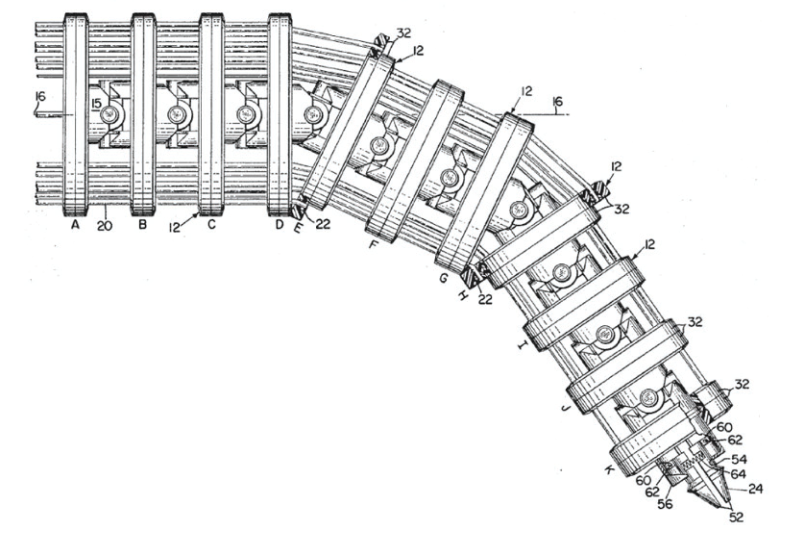
\includegraphics[width=.75\textwidth]{figures/tensor_arm.png}
	\caption{Tensor Arm机器人}
	\label{fig:tensor_arm}
\end{figure}
Ivanescu等建立了电流变液驱动的动力学模型并用滑膜方法和Bang-Bang方法进行了控制\cite{ivanescu_variable_1995}。本世纪前后,连续型机器人的研究取得了长远的进步。Clemson大学的Walker教授带领的研究团队对连续型机器人进行了广泛深入的研究,并研制了多款物理样机\cite{hannan_analysis_2001,gravagne_manipulability_2002,mcmahan_field_2006,walker_robot_2013,tonapi_next_2014,tonapi_novel_2015}。
新型连续型机器人的设计\cite{yigit_design_2017,conrad_interleaved_2017,qi_novel_2016}、运动学和动力学\cite{chikhaoui_kinematics_2016,godage_dynamics_2016}、控制和规划\cite{chikhaoui_kinematics_2016}等各方面的研究方兴未艾。

\section{连续型机器人的分类}
%	腱驱动、同心管、新型驱动(人造肌肉)与变刚度、软体机器人 。问题:轴向压缩回程间隙振动
%	传统的刚性结构机器人由于结构上不会发生柔性变形,因此可以通过有限个关节驱动其在三维空间运动;而连续型机器人的连续型弯曲变形

连续型机器人本质上可以是一种欠驱动机器人,其具有无限多自由度的弯曲变形仅能依靠有限多驱动源驱动,因此为了实现连续可控的弯曲变形,需要通过设计合适的机械结构和驱动方式进行对空间弯曲进行约束。
从驱动方式上看,连续型机器人一般可以分为腱驱动连续型机器人(Tendon-driven Continuum Manipulator)、同心圆管连续型机器人(Concentric Tube Continuum Manipulator)和新型驱动(如人工肌肉)机器人。
%	另外需要说明的是,软体机器人也是连续型机器人的一种\cite{robinson_continuum_1999},它们多采用腱驱动\cite{renda_3d_2012,renda_dynamic_2014}和新型驱动方式\cite{rus_design_2015,marchese_dynamics_2016,marchese_design_2016}。
\subsection{腱驱动机器人}
由于结构的限制,连续型机器人往往无法像传统机器人一样,将驱动单元直接与关节连接,而是通过绳子或弹性棒等柔性材料与位于机器人外部的驱动单元连接,远程驱动机器人弯曲变形,这类机器人属于腱驱动机器人。
%	这是一种外部驱动方式。
 
腱驱动连续型机器人的一般结构形式是由弹性支撑和均布于其四周的腱(绳子或弹性杆等),以及位于基座部位的驱动单元组成。机器人一般分为多节,每一节的末端有一组腱与之固连,驱动单元的驱动力经由腱传递到每一节的末端,从而使弹性支撑产生连续弯曲变形。图\ref{fig:tendril}中的Tendril机器人是典型的腱驱动机器人,它使用一系列可压缩弹簧作为弹性支撑,每个电机驱动一对绳子控制一个方向的弯曲\cite{mehling_minimally_2006}。
\begin{figure}[!htbp]
	\centering
	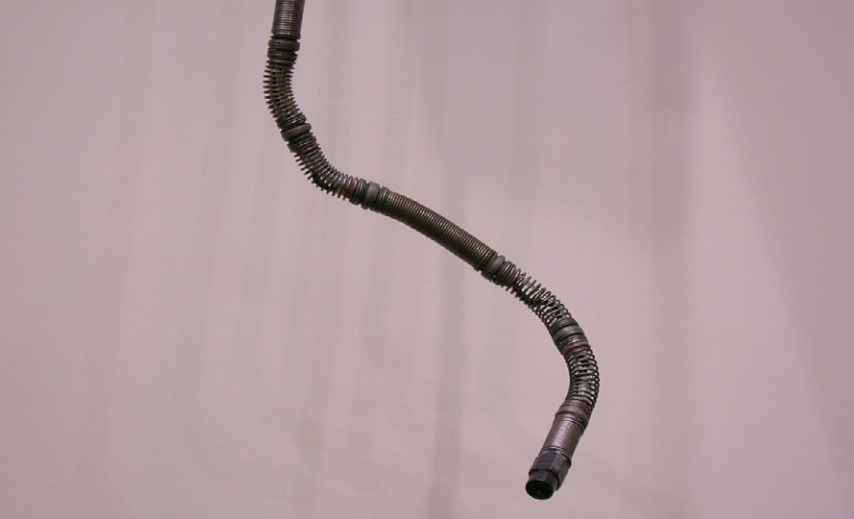
\includegraphics[width=.75\textwidth]{figures/tendril.png}
	\caption{Tendril机器人,腱驱动}
	\label{fig:tendril}
\end{figure}
 
这类机器人存在的主要问题有:
\begin{enumerate}
	\item 绳子的驱动力会同时会使得弹簧等可压缩弹性材料产生轴向压缩,导致弯曲变形和轴向压缩产生耦合,轴向压缩会导致弹性支撑刚度变大,柔顺性变差;
	\item 多节连续型机器人的驱动腱往往是利用过孔限制与机体一起变形,即后一节的驱动腱需要随前一节的变形而改变长度,造成了节间驱动的耦合,驱动误差会逐节累积放大,末端控制精度不高。
	\item 在往复运动过程中,绳子等单向施力的腱可能出现松弛\cite{hannan_kinematics_2003}和回程间隙\cite{bardou_control_2010}等问题。
\end{enumerate}
%	产生弯曲的另外,由于驱动每一节弹簧的绳子需要穿过其之前的部分,导致驱动误差(绳子长度的变化)逐节累积放大,造成了控制上产生很大的误差。
 
解决上述问题的思路有:
\begin{enumerate}
	\item 选择柔性不可压缩材料作为弹性支撑\cite{gravagne_large_2003,liu_development_2016,suh_design_2015,gao_workspace_2015}。例如MCMahan等设计了采用气压软管作为弹性支撑的Air-Octor机器人,通过气压变化控制弹性支撑的伸长和收缩,通过绳子控制弯曲\cite{mcmahan_design_2005}。Qi等设计了一种采用双层平面弹簧串联组成的连续型机器人,柔顺性分析表明,这种设计能够使得伸缩和弯曲解耦\cite{qi_novel_2014,qi_novel_2016};
	\item 
	将腱放置在机体外面,驱动器与力的作用点之间仅有腱连接,或实时估计变形对节间耦合造成的影响,进而补偿\cite{tonapi_novel_2015};
	\item 
	可以通过增加弹簧补偿机构\cite{hannan_kinematics_2003}或采取每根腱用一个电机驱动\cite{shang_design_2012}的方式解决松弛和回程间隙等问题。另外,将弹性棒同时作为腱和弹性支撑,既能解决了绳子作为腱会产生的问题,同时可以增加控制上的灵活性\cite{rone_mechanics_2014}。
	
\end{enumerate}
%	为了解决上述问题,一般选择柔性不可压缩材料作为弹性支撑\cite{gravagne_large_2003,liu_development_2016,suh_design_2015,gao_workspace_2015}。MCMahan等则设计了采用气压软管作为弹性支撑的Air-Octor机器人,通过气压变化控制弹性支撑的伸长和收缩,通过绳子控制弯曲\cite{mcmahan_design_2005}。Qi等设计了一种采用双层平面弹簧串联组成的连续型机器人,柔顺性分析表明,这种设计能够使得伸缩和弯曲解耦\cite{qi_novel_2014,qi_novel_2016}。

腱驱动连续型机器人的优点是设计思路比较简单,负载能力较强,因而得到了较广泛的研究,并出现了商业产品(OC机器人)。
%	但由于往往采用多节设计,腱可能出现松弛\cite{hannan_kinematics_2003}和回程间隙\cite{bardou_control_2010}的问题。这些问题可以通过增加弹簧补偿机构\cite{hannan_kinematics_2003}或采取每根腱用一个电机驱动\cite{shang_design_2012}的方式进行处理。Rone等将弹性棒同时作为腱和弹性支撑,解决了绳子作为腱会产生的问题\cite{rone_mechanics_2014}


\subsection{同心圆管机器人}
同心圆管机器人是另一种采用外部驱动的连续型机器人,一般是由多个具有高弹性材料(如Ni-Ti合金等)制作的同心圆管相互嵌套构成。
%	同心圆管之间可以相互滑动和绕同心轴旋转。
\begin{figure}[!htbp]
	\centering
	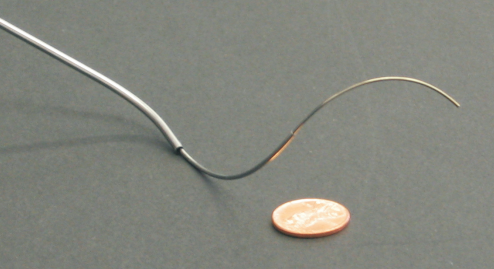
\includegraphics[width=.75\textwidth]{figures/ctm.png}
	\caption{同心圆管机器人\cite{webster_toward_2006}}
	\label{fig:ctm}
\end{figure}
 
同心圆管机器人可以实现长度上的伸缩和圆管绕同心轴的扭转,但受结构尺寸的限制,弯曲一般无法直接驱动。为了解决这个问题,一般将同心圆管进行预变形处理,这样具有初始曲率的内圆管在外圆管中滑动时,会在外圆管的的限制下发生弯曲变形\cite{sears_steerable_2006,webster_toward_2006,bergeles_concentric_2015,butler_robotic_2012}。

同心圆管机器人的机械设计上很简洁,并且由于主体部分只有相互嵌套的圆管,长细比可以非常大,常用于微创手术\cite{hendrick_hand-held_2015}等领域。该类机器人的缺点则包括载荷较小,弯曲无法直接驱动、工作空间较小等。
\subsection{具有新型驱动的连续型机器人}
与腱驱动机器人一样,同心圆管机器人的内圆管的弯曲变形与外圆管的形状参数有关,外圆管的变形直接对内圆管产生影响,因此采用外部驱动的连续机器人一般会存在节间耦合的问题,为了解决这一问题,许多采用内部驱动的新型驱动机器人被设计出来。
%	以上两种连续型机器人在采用多节设计是,后一节和前一节的驱动之间是相互耦合的。对于腱驱动来说,后一节的腱往往要穿过前一节的结构,前一节的结构变化就会使得在驱动后一节时要补偿掉前一节的该变量;对于同心圆管机器人来说,内圆管的弯曲变形是与外圆管的形状参数直接联系的,外圆管的变形直接对内圆管产生影响。为了解决这两种外部驱动存在的节间耦合的问题,研究这们设计了许多在节内部进行驱动的新型驱动机器人。
 
这类连续型机器人的驱动主要有气压(液压)人工肌肉、形状记忆合金\cite{ayvali_towards_2012-1}等。
气压(液压)人工肌肉是在气压或液压的作用下改变长度,进而驱动连接的端点发生伸缩、弯曲变形\cite{pritts_design_2004,guglielmino_octopus_2010}。OctArm(图\ref{fig:octarm})采用人工液压肌肉作为每一端点的驱动,成功进行了对不同形状目标的抓取和水下实验\cite{mcmahan_field_2006,trivedi_geometrically_2008}。
德国Festo公司的BHA机器人用波纹管是一种液压驱动的连续型机器人,它通过改变驱动波纹管的液压来说实现弯曲、伸缩\cite{falkenhahn_dynamic_2017}。Chikhaui等在同心圆管机器人的基础上添加了电活性聚合物(Electro-Active Polymers,EAP)作为控制器,从而实现对弯曲变形的主动控制\cite{chikhaoui_kinematics_2016}。
\begin{figure}[!htbp]
	\centering
	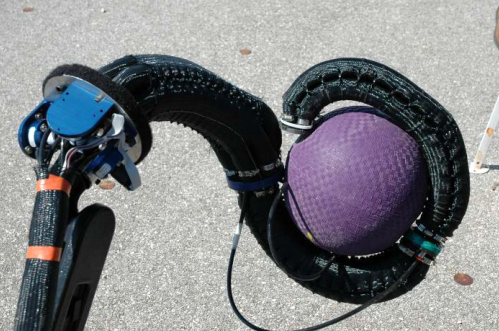
\includegraphics[width=.75\textwidth]{figures/octarm.png}
	\caption{OCtArm抓取物体实验\cite{mcmahan_field_2006}}
	\label{fig:octarm}
\end{figure}

内部驱动的连续型机器人能够直接驱动实现机器人的伸缩、弯曲、扭转变形,避免了其他两种连续型机器人的节间耦合,液压人工肌肉驱动等还能够产生较大的负载。这类机器人的缺点则是可能需要液压源和气压源,复杂的管道和阀门设计以及较高的加工装配精度。

\section{运动学}
和传统机器人运动学一样,连续型机器人的运动学一般也由三个空间之间的映射组成,即驱动空间、构型空间和任务空间。驱动空间与构型空间之间构成驱动运动参数(例如绳子长度变化)与连续型机器人形状参数(弯曲角度、弯曲方位)的映射关系,这一映射关系与机器人的设计有关,例如驱动方式不同,驱动空间参数一般也会不同;构型空间与任务空间构成形状参数与末端位姿之间的映射关系,这一映射与机器人设计无关\cite{webster_design_2010}。另一方面,运动学模型由结构参数直接决定的传统机器人不同,连续型机器人具有无限多自由度和内在的柔顺性,其结构参数在运动过程中是不断变化的,这种复杂性使得运动学建模方法成为了连续型机器人研究中的核心问题之一。
 
上述三类连续型机器人中,同心圆管机器人可以直接驱动嵌套圆管的滑动和伸长,不需要建立驱动空间与构型空间之间的映射。而对于采用腱驱动人工肌肉等新型驱动的连续型机器人,根据构型参数描述的空间变形采用几何学方法即可建立驱动空间与构型空间的映射关系\cite{jones_kinematics_2006,jones_practical_2006,webster_design_2010}。由于驱动空间与机器人的设计有关,因此目前并未有统一的建模方法。
%	下面主要针对构型空间与任务空间之间的映射关系进行介绍。
 
%	传统机器人的运动学模型由结构参数直接决定,而连续型机器人由于具有无限多自由度和内在的柔顺性,其结构参数在运动过程中是不断变化的,这种复杂性使得运动学建模方法成为了连续型机器人研究中的核心问题之一。
为了建立构型空间与任务空间的映射,一般采用几何的方法,通过对空间曲线的描述来建立二者之间的关系。在众多方法中,常曲率假设由于极大简化了运动学模型,因而在连续型机器人的建模中得到了广泛使用。
%	为了简化和近似描述连续型机器人的空间变形,一般假设机器人的形状具有常曲率。采用常曲率模型简化了运动学模型,易于实现多节的建模和逆运动学,在
%	同心圆管机器人可以直接驱动嵌套圆管的滑动和伸长,因此不需要建立驱动空间与构型空间之间的映射。而对于腱驱动机器人和人工肌肉等新型驱动机器人,根据构型参数描述的空间变形采用几何学方法即可建立驱动空间与构型空间的映射关系\cite{jones_kinematics_2006,jones_practical_2006,webster_design_2010}。
%	Tonapi等,采用实验数据建立变形与绳长变化的关系,对轴向压缩问题造成的误差进行了修正\cite{tonapi_novel_2015}.Camarillo等针对绳子松弛问题
%	采用优化的方法进行解决\cite{camarillo_configuration_2009}。
 
采用常曲率假设后,可以直接根据几何关系确定构型参数与机器人形状之间的关系\cite{bailly_modeling_2005,neppalli_design_2007}。还可以利用传统刚性机器人运动学建模所用的DH参数等工具。这种方法实际上是用离散的旋转和平移等效出连续型机器人上两点之间的位姿关系\cite{hannan_kinematics_2003,hannan_analysis_2001,walker_continuous_2013},对于平面连续型机器人,可以用旋转-平移-旋转三次操作来确定两点之间的位姿关系,对于空间运动,则可以用两次旋转一次平移和两次旋转进行确定\cite{hannan_kinematics_2003}。
 
虽然常曲率假设具有模型简单,计算量小的优点,但很多连续型机器人本质上无法产生常曲率的空间曲线。为了更精确的描述机器人的空间构型,需要考虑更为广泛的空间曲线表示方法。常用的方法有积分表示、模态函数等。积分表示是指表示出曲线上任一点切线的参数化坐标后,对其进行线积分以获得曲线上任一点的位置和空间指向\cite{chirikjian_hyper-redundant_1994,ivanescu_variable_1995}。模态函数则是用一系列基函数的线性组合来近似描述机器人的空间曲线,这类基函数包括三角函数\cite{chirikjian_modal_1994-1}、小波基函数\cite{gravagne_kinematics_2000}等。Godage等则直接用驱动空间参数的多项式对构型进行近似\cite{godage_shape_2011,godage_novel_2011,godage_dynamics_2016},从而之间建立了驱动空间与任务空间之间的映射关系。

 
另外,由于弹性体的变形和受力是紧密耦合的,因此在外力和扰动作用下,常曲率假设这种简单的几何假设可能不足以充分描述连续型机器人的运动学。Cosserat理论是对弹性介质在外力作用下变形的一个有力工具,利用Cosserat理论可以建立几何上比较精确地非常曲率运动学模型\cite{trivedi_geometrically_2008,jones_three_2009,rucker_geometrically_2010,mahvash_stiffness_2011,renda_general_2012}。但是这种模型计算上比较复杂,需要设计高效的计算方法才能够用于实时控制和模拟\cite{till_efficient_2015}。

%逆运动学?
一般来说,将上述方法建立的正运动学反解即可得到逆运动学\cite{sears_steerable_2006,camarillo_configuration_2009,neppalli_closed-form_2009},但由于连续型机器人具有的超冗余特性,即使采用常曲率假设进行简化也往往得不到解析解,需要采用数值计算方法\cite{jones_kinematics_2006,camarillo_mechanics_2008}。当机器人中存在非线性变形、未知干扰时,可以采用机器学习的方法学习逆运动学\cite{giorelli_feed-forward_2013,giorelli_neural_2015,rolf_efficient_2014,lakhal_hybrid_2016}。
%速度级运动学?


\section{动力学、控制和规划}
连续型机器人的动力学建模方法主要有牛顿-欧拉法\cite{khalil_dynamic_2007,kang_dynamic_2011}、拉格朗日方法\cite{mochiyama_kinematics_2003,godage_shape_2011,marchese_dynamics_2015,falkenhahn_dynamic_2015,godage_dynamics_2016}、集总参数法\cite{falkenhahn_dynamic_2015,falkenhahn_dynamic_2017,giri_three_2011,zheng_dynamic_2012}等。牛顿-欧拉法多用于模块化关节构成的连续风格的机器人,即有限自由度的机器人,而对于连续变形的具有无限自由度的机器人动力学建模来说,多采用拉格朗日方法。
%	与传统的刚性机器人不同,由于连续型机器人多由弹性材料组成,需要考虑材料变形中储存的弹性势能。
集总参数法多用于软体机器人和新型驱动机器人,是将弹性体等效为一个弹簧阻尼系统进行处理。连续型机器人的动力学模型与传统刚性机器人的区别主要是需要考虑弹性材料变形给结构参数带来的变化以及引入的弹性势能等。
 
%运动学、动力学、力、规划
由于连续型机器人难以像工业机器人等在关节处添加各种传感器,因此对其控制的研究大多是位置级。Qi等针对模型中存在不确定性,利用线性化后的状态空间模型建立了模糊控制器\cite{qi_kinematic_2016}。Marchese等设计了靠弹性材料局部膨胀实现弯曲的软体机器人的构型控制、正运动学算法等\cite{marchese_design_2016}。Yip等提出了一个任务空间的不依赖于模型的闭环控制器\cite{yip_model-less_2014},其思想是在线迭代估计机器人的雅克比矩阵。Chen等讨论了受限环境下基于传感器的位置引导控制方法\cite{chen_sensor-based_2009}。
%动力学
%	  
%	一般在建立连续型机器人的动力学模型后,会采用前馈控制对机器人的构型进行控制。
Falkenhahn等针对液压驱动的BHA机器人提出具有串联结构的前馈控制器\cite{falkenhahn_dynamic_2017}。Ivanescu等对非线性动力学解耦后采用滑膜控制策略对腱驱动连续型机器人进行了变形控制\cite{ivanescu_decoupled_2015}。Braganza等将神经网络作为前馈环节对OctArm进行动力学控制\cite{braganza_neural_2007}。
%力控
 
虽然连续型机器人具有柔顺性特点,特别适用于与环境存在交互的应用场合,但对这类机器人力柔顺的控制的研究还刚刚起步。
Bajo和Sim
aan提出了一种混合力位控制控制策略,并通过实验验证了该方法在连续型机器人与环境发生接触时的有效性\cite{bajo_hybrid_2016}。
%规划
%Chibani等提出了一个在约束环境下运动学构型的优化算法\cite{chibani_generating_2015}.
Goldman等用支持向量机估计标称模型中的非线性,设计了一种力柔顺策略\cite{goldman_compliant_2014}。Mahvash讨论了手术机器人的刚度控制,以实现末端指定力的输出\cite{mahvash_stiffness_2011}
